%% This is file AJCEAM-paper.tex is the template file for publications
%% in the "Academic Journal on Computing, Engineering and Applied Mathematics
%% from Universidade Federal do Tocatins, Brazil,
%% https://sistemas.uft.edu.br/periodicos/index.php/AJCEAM/index
%% This file was originally written by Tiago Almeida.
%% First revision: 2019-10-29
%% Second revision:
%%
%% History:
%%           2019-10-29 - First version by Tiago Almeida <tiagoalmeida@uft.edu.br>.
%%           2020-04-09 - English revision by Caio Machado <caio.machado@uft.edu.br>
%%

% Options
%     eng:   English Language
%     por:   Portuguese Language
%     blind: The version for reviewers is compiled (author data is hidden)


\documentclass[eng]{ajceam-class}
%
% Publication Title
\title{Modelado de la movilidad urbana en México con redes bayesianas}


% Short title for the header (copy the main title if it is not too long)
\shorttitle{Redes Bayesianas para la Movilidad Urbana}
       
% Authors
\author[1]{Diana L. Hernández-Almeida}
\author[1]{José A. López-Torres}
\author[1]{Axel D. Luna-Hernández}
\author[1]{Jorge E. Nevarez-Soto}

% Author Affiliations
\affil[1]{Tecnologico de Monterrey}

% Surname of the first author of the manuscript
%\firstauthor{Hernández, López, Luna and Nevarez}

%Contact Author Information
\contactauthor{Name A. Surname}           % Name and surname of the contact author
\email{name.surname@email.com}            % Contact Author Email

% Publication data (will be defined in the edition)
%\thisvolume{XX}
%\thisnumber{XX}

\thismonth{Octubre}
\thisyear{2024}

% Place your particular definitions here
\newcommand{\vect}[1]{\mathbf{#1}}  % vectors

% Insert here the abstract in English language
\abstract{
Urban mobility in Mexico is shaped by socioeconomic, demographic, and contextual factors that affect both transport mode choice and travel time. This study applies multinomial Bayesian networks to the 2017 Origin--Destination Survey (INEGI) to model these dependencies under uncertainty. Three candidate directed acyclic graphs (DAGs) were specified and fitted by maximum likelihood, and model fit was compared using BIC and AIC. The third DAG achieved the best fit (BIC = $-1{,}094{,}177$; AIC = $-985{,}745.9$) and was therefore selected as the reference model to address four policy-relevant questions: (i) the probability of automobile use by men traveling for religious purposes, (ii) the probability that trips longer than 60 minutes are motorized versus non-motorized, (iii) the probability that home-to-school trips exceed 60 minutes when school transport is used, and (iv) the probability of public transport use (bus, light rail, suburban rail) among high-stratum individuals in Cuauhtémoc borough on Saturdays. The results indicate that the probability of automobile use by men traveling for religious purposes is 20.6\%. For trips longer than 60 minutes, motorized transport strongly dominates, with a conditional probability of 80.9\% compared to 19.3\% for non-motorized modes. The probability that home-to-school trips exceed 60 minutes when school transport is used is very low, at 1.9\%. Finally, the probability that high-stratum individuals in Cuauhtémoc borough use public transport on Saturdays is also low, at 2.1\%. These findings highlight the usefulness of Bayesian networks to capture interdependencies in travel behavior and to inform evidence-based urban mobility planning.
}

% Insert here the keywords of your work in English language
\keywords{
Bayesian networks, transport, multinomial models, DAG, urban mobility, Mexico}


% Start document
\begin{document}

% Include title, authors, abstract, etc.
\maketitle
\thispagestyle{fancy}
%\printcontactdata



% Main body of manuscript
\section{Introduction}
\firstword{L}{a}% Capital letter in first word
movilidad urbana en México enfrenta el reto de explicar cómo factores sociodemográficos, económicos y contextuales determinan tanto la elección del modo de transporte como la duración de los viajes. Estudios previos han mostrado la influencia del estrato socioeconómico y el género en los patrones de movilidad, pero los enfoques tradicionales suelen ser insuficientes para capturar las complejas dependencias entre múltiples variables.

La Encuesta Origen Destino 2017 (INEGI) ofrece un panorama detallado de los motivos de viaje, tiempos de traslado y medios de transporte utilizados en áreas metropolitanas. En este trabajo, analizamos cómo el sexo, el estrato social, el día de la semana y motivaciones específicas como los viajes religiosos o escolares afectan la probabilidad de usar determinados modos de transporte y de realizar trayectos largos.

Para ello empleamos redes bayesianas multinomiales, una herramienta que permite representar relaciones de dependencia mediante grafos dirigidos y estimar probabilidades condicionales bajo incertidumbre. Nuestra hipótesis es que estas interacciones no lineales entre factores sociales y contextuales pueden modelarse de forma más precisa con este enfoque, generando evidencia útil para la planificación del transporte y la formulación de políticas públicas de movilidad.

\section{Metodología}

El trabajo se basó en el uso de redes bayesianas multinomiales para modelar dependencias entre variables sociodemográficas, contextuales y decisiones de transporte. El enfoque siguió un procedimiento reproducible en cuatro etapas principales.

En primer lugar, se realizó una limpieza del archivo Excel original de la Encuesta Origen--Destino 2017, seleccionando únicamente las variables necesarias para el análisis y generando un nuevo archivo en formato \texttt{.csv}. Esto permitió trabajar con una base de datos depurada y de menor tamaño, enfocada en los atributos relevantes para el estudio.

Posteriormente, las variables continuas se discretizaron en categorías de interés, entre ellas la duración de viaje mayor a 60 minutos (\texttt{dur\_60}). Las variables cualitativas se transformaron en factores categóricos para garantizar compatibilidad con los algoritmos de \texttt{bnlearn}\cite{scutari_bnlearn}, incluyendo: \texttt{sexo}, \texttt{acto\_religioso}, \texttt{motorizado}, \texttt{automovil}, \texttt{modo\_ok}, \texttt{es\_sabado}, \texttt{origen}, \texttt{estrato\_alto}, \texttt{st\_cuauh}, \texttt{destino} y \texttt{transporte\_escolar}.

De manera particular, la columna original \texttt{tra\_p5\_14}, que contenía información sobre los distintos modos de transporte, fue descompuesta en tres variables derivadas: \texttt{automovil} (uso o no de automóvil), \texttt{motorizado} (uso de cualquier modo motorizado) y \texttt{modo\_ok} (identificación de transporte público: autobús, tren ligero o tren suburbano). Una vez generadas estas variables, la columna original fue eliminada para evitar redundancias.

Posteriormente, se propusieron tres grafos acíclicos dirigidos (DAGs) que reflejaban hipótesis alternativas sobre las dependencias causales. Cada DAG fue implementado en el entorno \texttt{R} utilizando la librería \texttt{bnlearn}.


\subsection{DAG 1}

La DAG uno explica la siguiente relación: 
El uso de \texttt{automovil} está condicionado por la variable \texttt{sexo} y el \texttt{acto\_religioso}. 
La elección de transporte público (\texttt{modo\_ok}, que incluye autobús, tren ligero y tren suburbano) 
depende de \texttt{sexo}, \texttt{estrato\_alto}, \texttt{es\_sabado} y \texttt{acto\_religioso}. 
Tanto \texttt{automovil} como \texttt{modo\_ok} determinan si un viaje es \texttt{motorizado}. 
Finalmente, el hecho de ser \texttt{motorizado}, junto con \texttt{acto\_religioso} y \texttt{es\_sabado}, 
afecta la probabilidad de que el viaje dure más de 60 minutos (\texttt{dur\_60}).

\begin{figure}[H] 
 \centering
 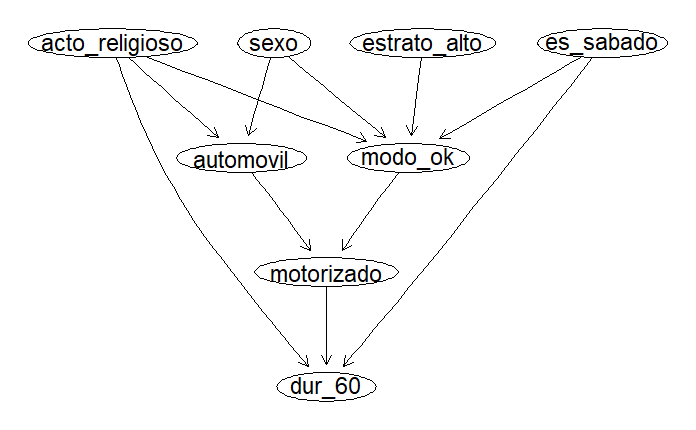
\includegraphics[width=0.8\columnwidth]{dag1} 
 \caption{Estructura propuesta para el DAG~1} \label{fig:dag1}
\end{figure}

\subsection{DAG 2}

La DAG dos explica la siguiente relación: 
La variable \texttt{automovil} depende de \texttt{sexo}, \texttt{estrato\_alto}, 
\texttt{acto\_religioso}, \texttt{es\_sabado}, \texttt{origen} y \texttt{destino}. 
La variable \texttt{modo\_ok} depende de \texttt{origen}, \texttt{destino}, 
\texttt{es\_sabado} y \texttt{estrato\_alto}. 
La condición de \texttt{motorizado} está determinada por \texttt{automovil} y \texttt{modo\_ok}. 
El \texttt{transporte\_escolar} depende de \texttt{estrato\_alto}, \texttt{origen} y \texttt{destino}. 
Finalmente, la duración del viaje (\texttt{dur\_60}) está influida por \texttt{origen}, 
\texttt{destino}, \texttt{modo\_ok}, \texttt{automovil}, \texttt{motorizado} 
y \texttt{transporte\_escolar}.

\begin{figure}[H] 
 \centering
 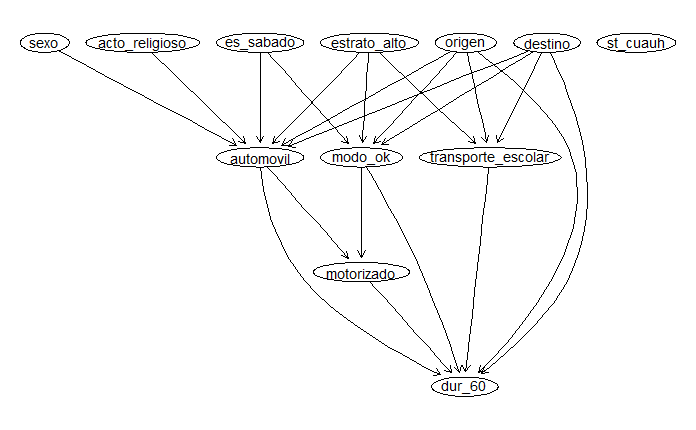
\includegraphics[width=0.8\columnwidth]{dag2} 
 \caption{Estructura propuesta para el DAG~2} \label{fig:dag2}
\end{figure}

\subsection{DAG 3}

La DAG tres explica la siguiente relación: 
La duración del viaje (\texttt{dur\_60}) depende de \texttt{automovil}, 
\texttt{motorizado} y \texttt{modo\_ok}. 
La variable \texttt{automovil} depende de \texttt{acto\_religioso}, 
\texttt{sexo}, \texttt{destino} y \texttt{estrato\_alto}. 
Las variables \texttt{motorizado}, \texttt{es\_sabado} y 
\texttt{transporte\_escolar} dependen de \texttt{destino}. 
El \texttt{destino} depende a su vez de \texttt{acto\_religioso}, 
\texttt{sexo} y \texttt{estrato\_alto}. 
Las variables \texttt{st\_cuauh} y \texttt{modo\_ok} dependen de 
\texttt{origen} y \texttt{estrato\_alto}, mientras que el \texttt{origen} 
depende de \texttt{estrato\_alto}.

\begin{figure}[H] 
 \centering
 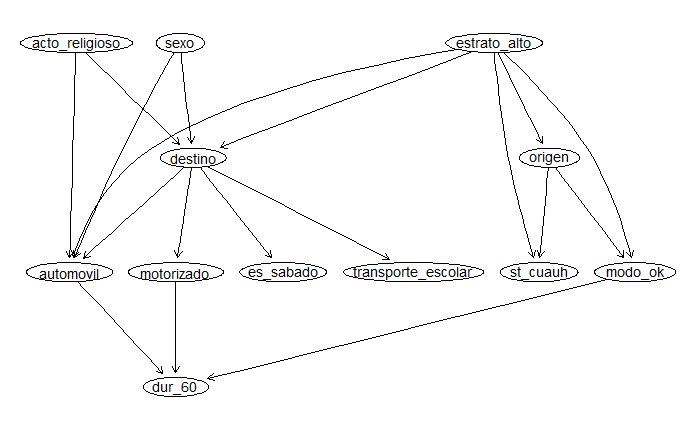
\includegraphics[width=0.8\columnwidth]{dag3}
 \caption{Estructura propuesta para el DAG~3.}
 \label{fig:dag3}
\end{figure}

\subsection{Evaluación de los modelos}

Se realizó el ajuste de parámetros por máxima verosimilitud para cada DAG mediante la función \texttt{bn.fit} del paquete \texttt{bnlearn}, y se evaluó el desempeño de cada estructura utilizando los criterios de información \textit{Bayesian Information Criterion} (BIC) y \textit{Akaike Information Criterion} (AIC). Adicionalmente, se utilizó la función \texttt{arc.strength} para comprobar la independencia condicional de los arcos y determinar cuáles dependencias resultaban significativas.

\begin{table}[H]
 \centering
  \caption{Criterios de información (BIC y AIC) obtenidos para cada DAG.} \label{tab:bic_aic}
 {\small
 \begin{tabular}{ccc}
  \hline
  \hline
  \thead{Modelo} & \thead{BIC} & \thead{AIC} \\
  \hline
  \hline
  DAG 1 & $-4447038$ & $-4443428$ \\
  DAG 2 & $-1484707$ & $-1163055$ \\
  DAG 3 & $-1094177$ & $-985745.9$ \\
  \hline
  \hline
 \end{tabular}}
\end{table}

Basándonos en estos valores, la DAG~3 presentó el mejor ajuste a los datos, al mostrar los puntajes de BIC y AIC menos negativos.

\subsection{Red bayesiana y Hill-Climbing}

Una vez seleccionada la DAG~3 como mejor estructura entre las propuestas, se convirtió en una red bayesiana completa mediante el ajuste de parámetros por máxima verosimilitud utilizando la función \texttt{bn.fit}. 

Adicionalmente, se aplicó el algoritmo \textit{Hill-Climbing} para aprender automáticamente la estructura a partir de los datos. Este enfoque obtuvo un mejor ajuste estadístico que las estructuras definidas manualmente, según los criterios BIC y AIC (véase Tabla~\ref{tab:hc}).

\begin{table}[H]
 \centering
  \caption{Criterios de información para la red aprendida con Hill-Climbing.}
  \label{tab:hc}
 {\small
 \begin{tabular}{ccc}
  \hline
  \hline
  \thead{Modelo} & \thead{BIC} & \thead{AIC} \\
  \hline
  \hline
  Hill-Climbing & $-943336.1$ & $-931741.8$ \\
  \hline
  \hline
 \end{tabular}}
\end{table}

Sin embargo, la red aprendida no siempre refleja relaciones causales plausibles en el contexto de la movilidad urbana, lo que limita su interpretabilidad. En consecuencia, el resultado de \textit{Hill-Climbing} debe considerarse únicamente como una referencia comparativa de ajuste.

\begin{figure}[H] 
 \centering
 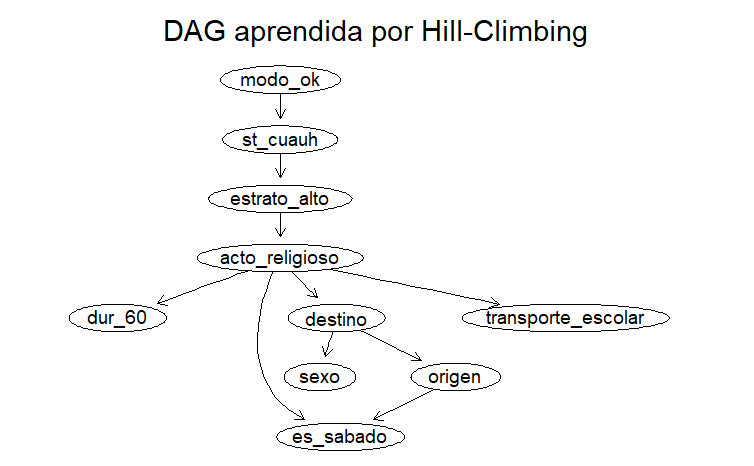
\includegraphics[width=0.8\columnwidth]{hc} 
 \caption{Estructura de la red aprendida mediante el algoritmo Hill-Climbing.}
 \label{fig:hc}
\end{figure}


\section{Aplicación}

La validación de los modelos se llevó a cabo a través del cálculo de probabilidades condicionales sobre escenarios de interés en movilidad urbana. Para ello se definieron cuatro consultas específicas, orientadas a responder preguntas de política pública y patrones de comportamiento: uso del automóvil en viajes religiosos (i), relación entre duración y transporte motorizado (ii), duración de viajes escolares (iii)y uso del transporte público en población de estrato alto en la alcaldía Cuauhtémoc durante fines de semana (iv).

\subsection{Uso del automóvil en viajes religiosos}

La primera consulta se planteó como: \textit{¿Cuál es la probabilidad de que el automóvil sea el medio de transporte de un hombre, dado que su propósito de viaje es asistir a un acto religioso?}

La probabilidad estimada de que un hombre utilice automóvil cuando el motivo del viaje es religioso fue de 20.6\%. Este resultado refleja que, aunque el automóvil se emplea en una parte de los desplazamientos hacia actividades religiosas, la mayoría de los viajes de este tipo se realizan mediante otros medios (posiblemente transporte público o caminata). Esto sugiere que el factor religioso no está fuertemente asociado con la elección del automóvil en comparación con otras variables contextuales.

\subsection{Duración de viaje y uso de transporte motorizado}

La segunda consulta buscó responder: \textit{¿Cuál es la probabilidad de que un viaje con duración mayor a 60 minutos se realice en transporte motorizado versus un viaje en transporte no motorizado?}

Condicionado a trayectos mayores a 60 minutos, la probabilidad de usar un medio motorizado es de 80.9\%, mientras que la probabilidad de utilizar un medio no motorizado es de apenas 19.3\%. Este hallazgo confirma la expectativa de que los viajes largos en la Ciudad de México dependen casi siempre de modos motorizados, dada la dificultad de sostener recorridos extensos a pie o en bicicleta. Además, la razón de probabilidades muestra una clara ventaja del transporte motorizado frente al no motorizado.

\subsection{Duración de viajes escolares}

La tercera consulta fue: \textit{¿Cuál es la probabilidad de que el viaje del hogar a la escuela dure más de 60 minutos si la persona utiliza transporte escolar?}

La probabilidad estimada de que un viaje del hogar a la escuela dure más de 60 minutos cuando se emplea transporte escolar es de apenas 1.9\%. Esto indica que, en la mayoría de los casos, el transporte escolar está asociado con recorridos relativamente cortos, probablemente debido a la planeación de rutas locales y a la cercanía entre las viviendas y los centros educativos.

\subsection{Uso de transporte público en estratos altos en Cuauhtémoc}

La cuarta consulta buscó determinar: \textit{¿Cuál es la probabilidad de que personas de estrato alto utilicen transporte público (tren suburbano, tren ligero o autobús) durante los sábados en la alcaldía Cuauhtémoc?}

La pregunta original se refería a individuos del estado de Zacatecas, pero la base de datos de la Encuesta Origen--Destino 2017 incluye únicamente trayectos dentro de la Ciudad de México. Por lo tanto, se ajustó la consulta para mantener la coherencia con la información disponible, reemplazando Zacatecas por la alcaldía Cuauhtémoc.

La probabilidad calculada de que personas de estrato alto en Cuauhtémoc utilicen transporte público en sábado es de 2.1\%. Este valor, muy bajo, refleja la fuerte preferencia de los sectores de mayor ingreso por modos privados de transporte, principalmente el automóvil, y sugiere desigualdades persistentes en el acceso y uso del transporte público.

\section{Conclusiones}
El estudio aplicó redes bayesianas multinomiales para analizar la movilidad urbana en la Ciudad de México a partir de la Encuesta Origen--Destino 2017. Se evaluaron tres estructuras iniciales y se compararon con el algoritmo Hill-Climbing. Aunque este último alcanzó mejores valores de ajuste estadístico, generó relaciones poco plausibles, por lo que la estructura de la DAG~3 se consideró más adecuada para la interpretación de los datos.

Las consultas realizadas mostraron patrones consistentes. La probabilidad de que un hombre use automóvil en viajes religiosos resultó baja, mientras que en trayectos de más de una hora predominó el transporte motorizado. El transporte escolar presentó una probabilidad mínima de viajes largos, lo que refleja su carácter local, y la población de estrato alto en la alcaldía Cuauhtémoc mostró un uso muy reducido del transporte público durante los sábados.

Estos hallazgos confirman la existencia de desigualdades en la elección modal y destacan el valor de los enfoques probabilísticos para representar interdependencias complejas en la movilidad urbana. Entre las principales limitaciones se encuentra la necesidad de discretizar y simplificar variables, lo que puede restringir el nivel de detalle capturado. Futuros trabajos deberían ampliar el conjunto de variables consideradas y explorar técnicas que combinen un buen ajuste estadístico con mayor coherencia causal y contextual.

% Include references
\insertbibliography{References}


\end{document}
